%----------------------------------------------------------------------------
%bb defines the bounding box for the pdf
%viewport defines the area of the pdf used
%in sidewaysfigure the last entry in bb moves the caption toward/away the pic
%in sidewaysfigure the second entry in bb moves the pic toward/away the caption
%----------------------------------------------------------------------------
\begin{figure}
\begin{center}
\leavevmode
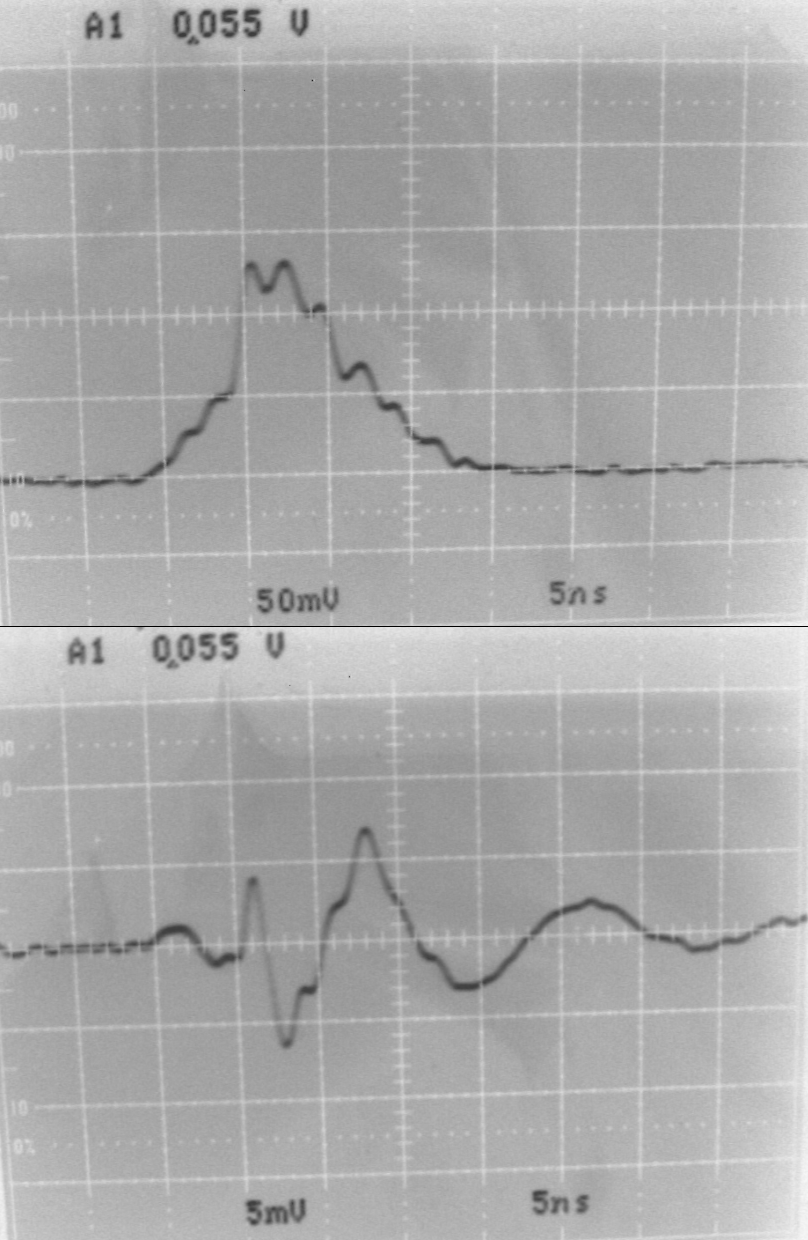
\includegraphics[width=4in]
{filter/filter.png}\\
\end{center}
\caption[Photodiode signal through the highpass filter (and 14 dB attenuator)]{Photodiode signal through the highpass filter (and 14 dB attenuator). The upper photo shows a typical signal from the photodiode after a dye laser pulse is detected. The lower photo shows a typical signal after the insertion of the 14 dB attenuator and the highpass filter between the photodiode and the oscilloscope.}
\label{filter}
\end{figure}
%----------------------------------------------------------------------------
